When presented a motion sequence, moving hand is first detected in each image of the sequence. This is done in a number of steps.

At first image background is subtracted from the image. This allows us to only see what has changed in the image comparing to the background. Example of image from which background was subtracted is shown in Figure \ref{fig:bgsub}.

\begin{figure}
\begin{center}
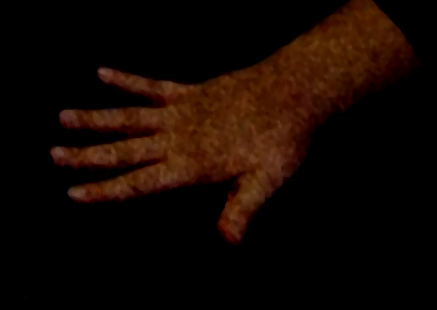
\includegraphics[width=80mm]{bgsub.png}
\caption{Image obtained by performing background subtraction.}
\label{fig:bgsub}
\end{center}
\end{figure}


Obtained image is then smoothened using median blur in order to reduce noise. Such image is then transformed into black and white image according to threshold based on a colour difference between a typical hand in the data set and the background of the image. Such colour is found to lie between RGB values of $(0, 0, 27)$ and $(100, 100, 140)$. Image obtained by thresholding is shown in Figure \ref{fig:bw}.

\begin{figure}
\begin{center}
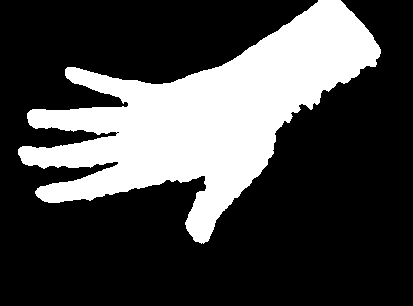
\includegraphics[width=80mm]{bw.png}
\caption{Image obtained by thresholding preprocessed image.}
\label{fig:bw}
\end{center}
\end{figure}


To improve precision of the background subtraction and to account for possible lighting changes between different sets of images, first image of the sequence is also subtracted from the image. This removes all static features from the motion sequence. Such static features are often artifacts caused by changed lighting conditions between different the times different motion images were made. Both, the first image which is subtracted from the image of interest and the image of interest itself, are preprocessed in the same way.

\begin{math}
Image^*_n = f(Image_n - Background) - f(Image_1 - Background), n \geq 2
\end{math}

Dilation is then performed on such image. This helps further smoothen the detected hand and also helps eradicate any noise which appears not attached to the hand. Furthermore, dilation helps to connect parts of the same object which might appear disjoint because of shadows. This is often the case in images of hand showing "scissors" sign, where two fingers do not appear connected in the processed image because of a shadow between fingers.

Contours of the objects are then detected using simple chain approximation algorithm. Such algorithm scans binary image vertically as well as horizontally looking for chains of white pixels. It flips all the white pixels except from the pixels which represent both ends of each such chain. Using this technique we are able to obtain contours of all objects in the image. Contours of object obtained by using this method is showin in Figure \ref{fig:contours}.

\begin{figure}
\begin{center}
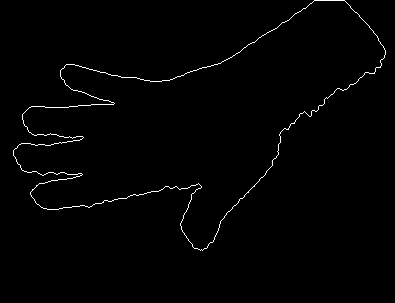
\includegraphics[width=80mm]{contours.png}
\caption{Image obtained by using simple chain approximation algorithm.}
\label{fig:contours}
\end{center}
\end{figure}

Largest object in the image is then chosen. If area of such object is above given threshold, the object is chosen as representation of the hand in the image, this helps not include initial and last images of the hand in the sequence where it is not fully visible in the picture.

Summary of the algorithms and parameters used in the Hand Recognition module is presented in Table \ref{tbl:recognition}.

\begin{table}
\begin{tabular}{|c|l|}
\hline 
Preprocessing: & Smoothing with Median blur  Background subtraction\\ 
\hline 
Background subtraction: & Using background image provided\\ 
\hline
Thresholding: & on RGB image, $(0, 0, 27)$ and $(100, 100, 140)$\\ 
\hline
First image subtraction: & subtracting first image of the sequence\\ 
\hline
Mathematical Morphology & Dilation using Cross Kernel of size 11 $\times$ 11 \\ 
\hline 
Contour Extraction: & Simple Chain Approximation \\ 
\hline 
Area measure: & discarding contours of small size \\
\hline 
\end{tabular} 
\caption{Summary of Classification Module parameters and algorithms}
\label{tbl:recognition}
\end{table}